\documentclass[12pt]{article}

\usepackage{template_wete}
\usepackage{ifthen}

\usepackage{graphicx,url}
\usepackage{multirow} %% essencial %% para uso de tabelas
\usepackage{supertabular} %% essencial %% para uso de tabelas
\usepackage{tabularx} %% essencial %% para uso de tabelas
\usepackage{longtable}
\usepackage{gensymb}
\usepackage{color}
\usepackage{fancyhdr}
\usepackage[english]{babel}   
%\usepackage[latin1]{inputenc}


\fancypagestyle{plain}{%
\fancyfoot[LE, RO]{Apurba Paul}
\fancyfoot[LO, RE]{Using fancyhdr}}


%------------------------------------------------------------------------------------------ CABEÇALHOS
\sloppy
\title{Analysis of Damage Costs on 150cc Motorcycles on 2,500 Feet Mountain Roads}

\author{Lucas Siva e Silva\inst{1}, Kim Impossible\inst{2}, Dino da Silva Sauro\inst{1}, Jomi F. Hübner\inst{3} }


\address{Instituto Nacional de Pesquisas Espaciais\\
  Aluno de Mestrado do curso de Ciência e Tecnologia de Materiais e Sensores - CMS
\nextinstitute
  Department of Computer Science -- University of Durham\\
  Durham, U.K.
\nextinstitute
  Departamento de Sistemas e Computação\\
  Universidade Regional de Blumenal (FURB) -- Blumenau, SC -- Brazil
  \email{\{lucas,dino\}@inpe.br, kim@possible.br,
  jomi@inf.furb.br}
}


%\pagestyle{fancy}
\renewcommand{\headrulewidth}{0pt}
\renewcommand{\footrulewidth}{0pt}
\fancyhead{}
\fancyfoot{}

\fancyhead[C]{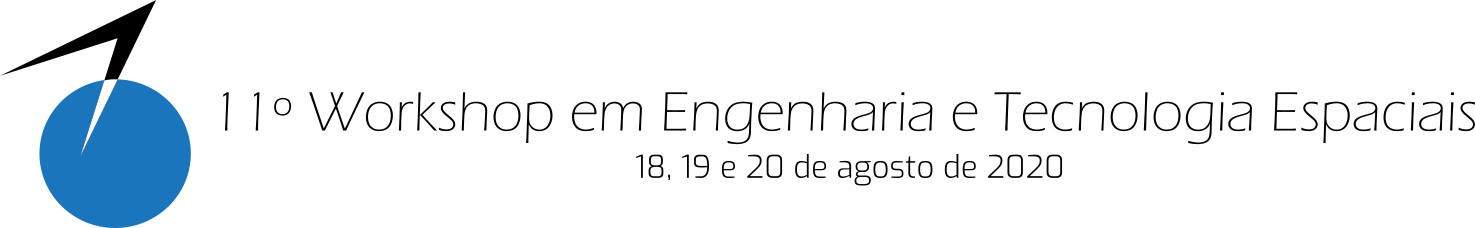
\includegraphics[width=13cm]{logo_template.png}}
\vspace{3.7cm}

%------------------------------------------------------------------------------------------ CABEÇALHOS

%------------------------------------------------------------------------------------------ CORPO DO TEXTO
\begin{document} 

\maketitle

\begin{abstract}
This study investigates the maintenance costs and mechanical damage associated with using 150cc motorcycles on mountain routes with an elevation of 2,500 feet (approximately 762 meters). Through theoretical stress analysis and estimation of component wear, it was identified that thermal stress and mechanical overload result in significant repair costs, focusing mainly on the clutch system, brakes, and lubricating oil degradation.
\end{abstract}
\hrulefill

\begin{flushleft}
\textbf{Keywords:} 150cc Motorcycle; Maintenance Cost; Mountain Climbing; Mechanical Wear; Automotive Engineering.
\end{flushleft}

\section{Introduction}

Motorcycles with a displacement of 150cc are widely used in urban transport and rural roads due to their energy efficiency and cost-benefit. However, when subjected to extreme conditions, such as ascending mountains with 2,500 feet of altitude on motorable roads, these vehicles operate outside their ideal torque and rotation range \cite{cossalter2006}.

Prolonged effort on steep inclines requires the engine to operate at high RPMs for long periods, resulting in increased temperature and stress on mechanical components. Furthermore, frequent use of the clutch to maintain stability at low speeds and overload on the braking system during descent are critical factors for premature wear.

The objective of this work is to quantify potential damages and estimate repair costs associated with this specific activity, providing subsidies for motorcyclists and fleet managers regarding economic viability and maintenance risks.

\section{Methodology} \label{sec:met}

The methodology employed is based on a qualitative and quantitative analysis of the mechanical stresses imposed on a standard 150cc motorcycle (air-cooled, 4-stroke) during a simulated climb of 2,500 feet.

The following parameters were considered:
\begin{itemize}
    \item \textbf{Thermal Analysis:} Estimation of the temperature rise of the engine and lubricating oil based on workload and air resistance.
    \item \textbf{Clutch Wear:} Calculation of the friction work performed by the clutch system during starting and maintaining speed on inclines greater than 10\%.
    \item \textbf{Braking System:} Evaluation of brake pad and disc wear considering gravitational force during descent.
    \item \textbf{Parts Costs:} Survey of average market prices (in USD) for replacement of critical components (clutch kit, pads, oil, filters).
\end{itemize}

Reference data were obtained from maintenance manuals of popular manufacturers and specialized literature on two-wheeled vehicle dynamics \cite{kumar2022}.

\section{Resultados e Discussão}

Na seção Resultados e Discussão é apresentado o resultado, o que corresponde ao desenvolvimento do trabalho. Os resultados da investigação devem ser apresentados de forma clara, atendendo às características do tipo de dados obtidos. 

É nesse item que os dados da pesquisa são interpretados, criticados e comparados com os já existentes sobre o assunto na literatura citada; são discutidas suas possíveis implicações, significados e razões para concordância ou discordância com os autores. A discussão deve fornecer elementos para a conclusão. É o mais livre dos itens e o que mais evidencia a vivência do pesquisador. Se apropriado, podem ser inseridas tabelas (Tabela~\ref{tab:exemploTab1}) e figuras (Figura~\ref{fig:exemploFig1}) das análises feitas.


\begin{longtable}{l l l}
\caption{Exemplo de Tabela. \textcolor[rgb]{1,0,0}{[Fonte: se aplicável]}}\\
\hline
\textbf{Cidade} & \textbf{Temperatura (\celsius)} & \textbf{Umidade Relativa (\%)} \\
\hline
\endfirsthead
\multicolumn{3}{c}%
{\tablename\ \thetable\ -- \textit{Continuado da página anterior.}} \\
\hline
\textbf{Cidade} & \textbf{Temperatura (\celsius)} & \textbf{Umidade Relativa (\%)} \\
\hline
\endhead
\hline \multicolumn{3}{r}{\textit{Continua da próxima página.}} \\
\endfoot
\hline
\endlastfoot

Taubaté & 26 & 43\\
Ilhéus & 34 & 85

\label{tab:exemploTab1}
\end{longtable}


\begin{figure}[ht]
\centering
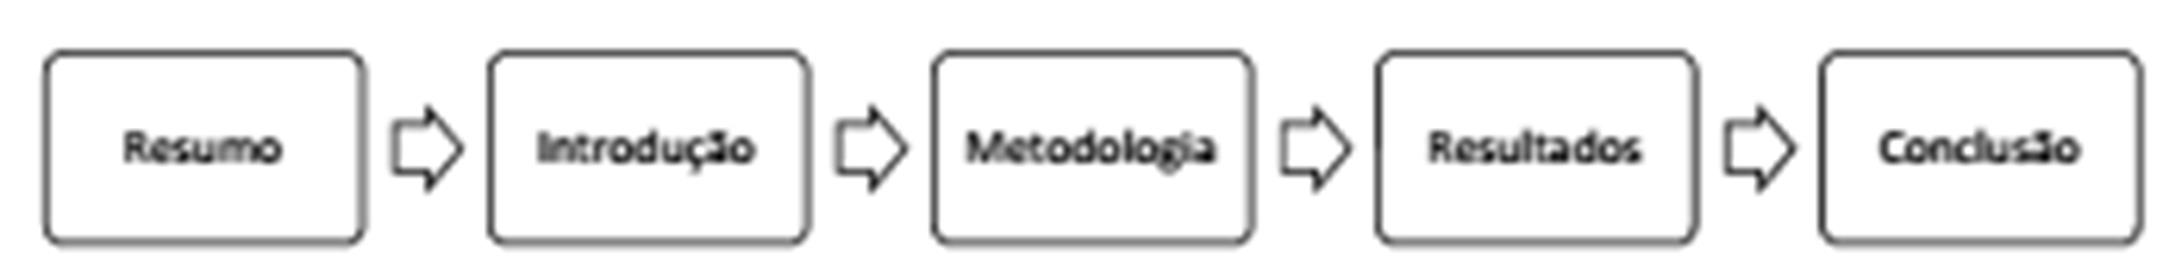
\includegraphics[width=\textwidth]{figura.jpg}
\caption{Exemplo de figura. \textcolor[rgb]{1,0,0}{[Fonte: se aplicável]} }
\label{fig:exemploFig1}
\end{figure}

\section{Conclusão}
Constitui o fecho do trabalho e deve ser breve e fundamentada nos resultados obtidos. Deve retornar ao objetivo, inicialmente proposto na seção Introdução, para analisar o quanto foi ou não alcançado. 

As referências devem conter apenas as bibliografias citadas como: \cite{knuth:84}, \cite{boulic:91} e \cite{smith:99}.


\begin{flushleft}
\emph{\textbf{Acknowledgments:} Item intended to inform funding agencies, supporting institutions, and collaborators. \textcolor[rgb]{1,0,0}{(OPTIONAL)}}
\end{flushleft}

%------------------------------------------------------------------------------------------ CHAMA AS REFERÊNCIAS
\bibliographystyle{ref_wete}
\bibliography{referencias}

%------------------------------------------------------------------------------------------ RETIRAR DA VERSÃO FINAL:
\textcolor[rgb]{1,0,0}{
IMPORTANTE: (remover na versão final)
\begin{itemize}
	\item Número de páginas: O trabalho deve conter no \textbf{MÍNIMO 4} e no \textbf{MÁXIMO 10} páginas;
	\item Autor para correspondência: Deve ser apresentado apenas 1 e-mail para correspondência;
	\item Citações: As citações devem ser feitas seguindo o padrão: [SOBRENOME DOS AUTORES ANO];
	\item Os autores devem se atentar às citações para não cometer o plágio;
	\item Referência: A seção Referências deve ser apresentada em ordem alfabética;
	\item Identificação dos Autores: 
	\item Na descrição o autor deverá informar a situação acadêmica atual (ex: aluno de mestrado/doutorado, mestre ou doutor) e a área de concentração da ETE a qual está vinculado. Ver exemplo abaixo.;
	\item Agradecimentos: Se o primeiro autor for bolsista (CAPES, CNPq, FAPESP, entre outras), o mesmo deverá citar a agência financiadora no item Agradecimentos.
\end{itemize}
%\small{
Identificação:\\\\
Para alunos do INPE:\\
Nome completo\\
Situação do aluno (Mestrando/Doutorando)  na PG-ETE e a área de concentração. Exemplo: Mestrando em Engenharia e Gerenciamento de Sistemas Espaciais\\
Instituto Nacional de Pesquisas Espaciais\\\\
Para orientadores (INPE):\\
Nome completo\\
Divisão / Departamento que atua no INPE\\
Instituto Nacional de Pesquisas Espaciais\\\\
Para Orientadores (externos ao INPE):\\
Nome completo\\
Departamento que atua\\
Instituição de Ensino / Empresa\\\\
Para alunos de Iniciação Científica:\\
Nome completo\\
Iniciação Científica na Divisão xxxxx\\
Instituto Nacional de Pesquisas Espaciais\\
%}
}
\end{document}
%------------------------------------------------------------------------------------------ CORPO DO TEXTO